\chapter{绪论}
\section{选题背景}
无人机(Unmanned Aerial Vehicle)即无人驾驶飞行器,广义上为不需要驾驶员驾驶的空中飞行器。过去,无人机常用于民事和军事行动,如救援和搜索、气候监测、监视、天气预报和绘图。自从现代技术的发展和互联网的创新以来,无人机已经发生了彻底的变化。如今,无人机还用于风暴、洪水和丛林火灾等自然灾害期间的紧急疏散。除此之外,无人机还广泛应用于民用建筑和航拍中,例如将材料运送到施工现场无法到达的位置,以及监测已建建筑以发现损坏,以实现智能城市的目的,在房地产管理和智慧城市的各个领域的使用也在增加。

% \begin{figure}[H]
%     \vspace{12pt}   
%     \centering
%     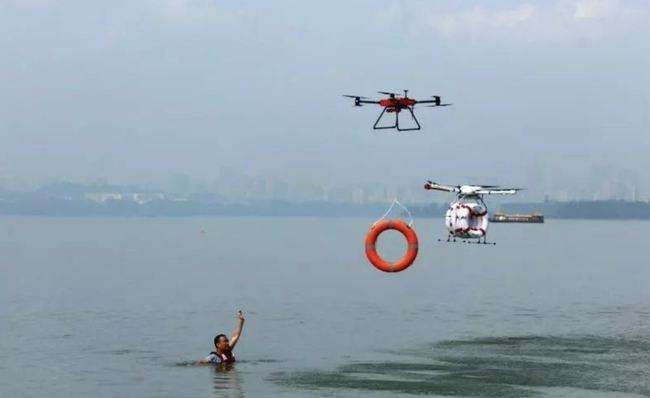
\includegraphics[width=12cm]{figures/fig_uvafun.png}
%     \caption{
%         无人机救援
%     }
%     \label{f1}
% \end{figure}
\begin{figure}[H]
    \vspace{12pt}  
    \centering
    \subfloat[运输]{
    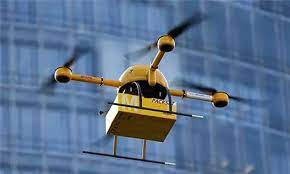
\includegraphics[width=6cm]{figures/fig_uvatransport.jpg}
    }
    \quad
    \subfloat[摄影]{
    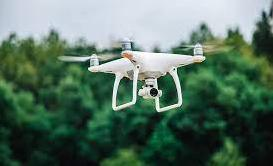
\includegraphics[width=6cm ]{figures/fig_uvashoot.jpg}
    }
    \quad
    \subfloat[监测]{
    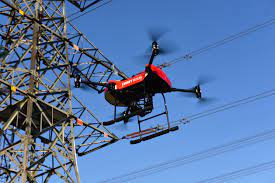
\includegraphics[width=6cm]{figures/fig_uvainspection.jpg}
    }
    \quad
    \subfloat[喷洒]{
    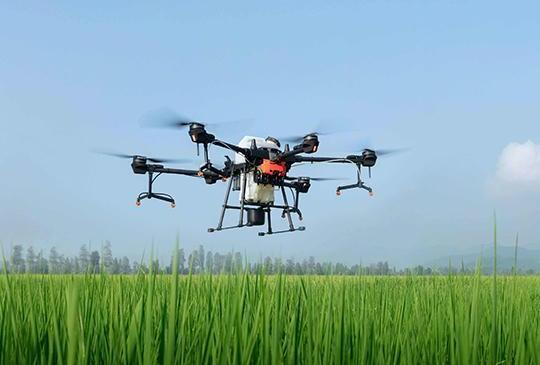
\includegraphics[width=6cm ]{figures/fig_uvafarm.jpg}
    }
    \caption{ 无人机应用}
    
\end{figure}


\section{研究现状}

随着无人机的应用领域越来越广泛,对于在一些高维、复杂和未知环境中飞行的无人机,安全变得至关重要。路径规划作为无人机飞行的关键技术,越来越受到研究者的重视。目前现有的适合无人机的路径搜索算法和路径优化方法大致如图 \ref{fig2} 所示。
\begin{figure}[H]
    \vspace{12pt}
    \centering
    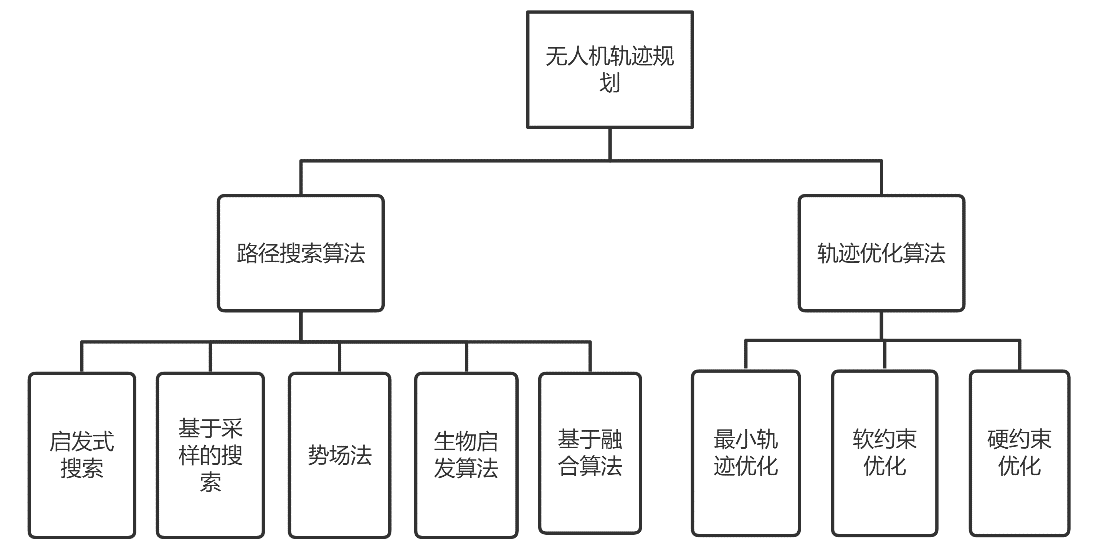
\includegraphics[width=12cm]{figures/fig2.png}
    \caption{
        常用算法
    }
    \label{fig2}
\end{figure}

\subsection{路径搜索算法}



\subsection{轨迹优化算法}


\section{本文研究内容}





\endinput
